\documentclass[]{article}
\usepackage{lmodern}
\usepackage{amssymb,amsmath}
\usepackage{ifxetex,ifluatex}
\usepackage{fixltx2e} % provides \textsubscript
\ifnum 0\ifxetex 1\fi\ifluatex 1\fi=0 % if pdftex
  \usepackage[T1]{fontenc}
  \usepackage[utf8]{inputenc}
\else % if luatex or xelatex
  \ifxetex
    \usepackage{mathspec}
  \else
    \usepackage{fontspec}
  \fi
  \defaultfontfeatures{Ligatures=TeX,Scale=MatchLowercase}
\fi
% use upquote if available, for straight quotes in verbatim environments
\IfFileExists{upquote.sty}{\usepackage{upquote}}{}
% use microtype if available
\IfFileExists{microtype.sty}{%
\usepackage[]{microtype}
\UseMicrotypeSet[protrusion]{basicmath} % disable protrusion for tt fonts
}{}
\PassOptionsToPackage{hyphens}{url} % url is loaded by hyperref
\usepackage[unicode=true]{hyperref}
\hypersetup{
            pdfborder={0 0 0},
            breaklinks=true}
\urlstyle{same}  % don't use monospace font for urls
\usepackage[margin=1in]{geometry}
\usepackage{longtable,booktabs}
% Fix footnotes in tables (requires footnote package)
\IfFileExists{footnote.sty}{\usepackage{footnote}\makesavenoteenv{long table}}{}
\usepackage{graphicx,grffile}
\makeatletter
\def\maxwidth{\ifdim\Gin@nat@width>\linewidth\linewidth\else\Gin@nat@width\fi}
\def\maxheight{\ifdim\Gin@nat@height>\textheight\textheight\else\Gin@nat@height\fi}
\makeatother
% Scale images if necessary, so that they will not overflow the page
% margins by default, and it is still possible to overwrite the defaults
% using explicit options in \includegraphics[width, height, ...]{}
\setkeys{Gin}{width=\maxwidth,height=\maxheight,keepaspectratio}
\IfFileExists{parskip.sty}{%
\usepackage{parskip}
}{% else
\setlength{\parindent}{0pt}
\setlength{\parskip}{6pt plus 2pt minus 1pt}
}
\setlength{\emergencystretch}{3em}  % prevent overfull lines
\providecommand{\tightlist}{%
  \setlength{\itemsep}{0pt}\setlength{\parskip}{0pt}}
\setcounter{secnumdepth}{0}
% Redefines (sub)paragraphs to behave more like sections
\ifx\paragraph\undefined\else
\let\oldparagraph\paragraph
\renewcommand{\paragraph}[1]{\oldparagraph{#1}\mbox{}}
\fi
\ifx\subparagraph\undefined\else
\let\oldsubparagraph\subparagraph
\renewcommand{\subparagraph}[1]{\oldsubparagraph{#1}\mbox{}}
\fi

% set default figure placement to htbp
\makeatletter
\def\fps@figure{htbp}
\makeatother


\author{}
\date{\vspace{-2.5em}}

\begin{document}

\begin{longtable}[]{@{}l@{}}
\toprule
title: ``Kandidat Skrivandet''\tabularnewline
author: ``Anton Holm''\tabularnewline
date: `2020-02-24'\tabularnewline
output:\tabularnewline
pdf\_document: default\tabularnewline
word\_document: default\tabularnewline
html\_document: default\tabularnewline
\bottomrule
\end{longtable}

\subsection{Abstrakt}\label{abstrakt}

\subsection{Introduction}\label{introduction}

\begin{itemize}
\tightlist
\item
  Maybe add graph to show how censored data looks like? So 2 graphs, one
  how it actually is, one how it's reported.
\item
  Show that the museum data is log-linear
\end{itemize}

\subsection{Background}\label{background}

At the Swedish Museum of Natural History, the Department of
Environmental Research and Monitoring in a joint effort with other
departments conducts statistical research of environmental toxicants as
part of the National Swedish Contaminant Programme in marine biota. One
of the programs conducted regards analysing long term time trends of
several toxins in Swedish waters and to estimate the rate of change. The
models used to analyse such time trends are at the moment surprisingly
elemental and disregards much of the data collected. One of the more
common, but nonetheless crucial oversights, concerns building models and
drawing conclusions from fabricated data due to data being censored.

\subsection{Data}\label{data}

The report from Bignert at al (2017) explains much of the data sampling.
The data comes from several sampling areas regarded as locally
uncontaminated. Several species of fish, as well as guillemot eggs and
blue mussels, are collected from different sampling areas each year.
When collected, a constant number of 10-12 speciemens independent of
each other are analysed for a large number of toxins. For some species,
the analysis is done for pooled samples containing a number of
speciemens in each pool. To reduce the between-years variation, each
sampling area tries to analyse speciemens of the same sex and age.
However, the variation can not be reduced to zero and other parameters
effects the variation such as fat content and local discharges as an
example. The concentration between each fish will also contain noise,
hence the data sampled will have variation between years as well as
within years.

As a result of test equipments not being able to detect small enough
quantities of toxins, a portion of the data is reported as \emph{below
the limit of quantification (LOQ)}. This portion of the data is reported
as the LOQ divided by the square root of 2.

Due to biological properies such as size and fat tissues being able to
effect the concentration of toxins and these attributes being effected
by sampling site, this thesis will analyse sampling areas individually.

Bignert at al (2017) uses log-linear regression analysis, hence the data
is assumed to follow a log-linear distribution.

\subsection{Common Errors}\label{common-errors}

One of the most common error being made when analysing censored data is
fabricating. The analysists simply substitute the non-detects with a
fraction (often one half) of the quantitive- or detetection limit. A
simulation were made by Helsel (2006) showcasing that this method
produces lousy estimates of statistics and have the potential to not
only overlook patterns in the data, but also impose it's own fabricated
patterns. This could result in a goverment investing millions to clean a
lake of toxins after a report displaying an increase in concentrations
of a certain metal in fish when in fact, there were no such pattern to
begin with. The reverse is even more terrifying, obtaining a report
showing no significant increase in concentration, when indeed the
concentration of said metal have been increasing for years. Causes of an
increase in concentration have been missed, remediations goes undone and
the health of humans and the ecosystem is unnecessarily endangered.
There are plenty more mistakes commonly being made when handling
censored data including misinterpreting an improvement in measuring
technique for a decrease in non-detects. However, this will not be
discussed in detail in this thesis.

\section{Theory}\label{theory}

When working with censored data, the non-detects can't be looked at as
having a specific value. Instead, a combination of the information of
the proportion of non-detects with the numerical values of the
uncensored observations gives a better understanding of the data.
Assuming a distribution for the data above and below the reported limit
in combination with the above mentioned information gives a foundation
to work with maximum likelihood estimates (MLE). In a study of Chung
(1990) regarding regression analysis of geochemical data with
non-detects, it was shown that MLE gave a much better estimation for the
true value of the slope coefficient than any of the substitution values
(0, 0.1, \ldots{}, 1 times the detection limit). Regression analysis for
censored data is being used in many fields, including but not limited
to, medical statistics as used by Lee and Go (1997) and in economics
where Chay and Honore (1998) used MLE regression on right-censored data
to model incomes. However, for left-censored data where the residuals is
assumed to follow a normal distribution, the MLE regression is sometimes
mentioned as Tobit analysis after the famous economist James Tobin. For
the particular data from the Museum of Natural History, the use of Tobit
regression models can serve useful to handle the censoring while the use
of a Linear Mixed-Effect Model (LMM) will deal with the fact that data
contains variation both within and between years.

\subsection{CDF of a linear regression
model}\label{cdf-of-a-linear-regression-model}

Consider a normal simple linear regression model \[
y_i = x_i \beta + \epsilon_i, \; \epsilon_i \sim N(0,\sigma^2)
\]

were \(y_i\) is the response variable, \(x_i\) the explanatory variable,
\(\beta\) an effect parameter and \(\epsilon_i\) the error term. It's
then easy to find the cumulative distribution function (CDF) for this
model.

\[
F(y_i) = P(x_i\beta+\epsilon_i\leq y_i) = P(\frac{\epsilon_i}{\sigma}\leq \frac{1}{\sigma}(y_i-x_i\beta)) = \Phi[\frac{1}{\sigma}(y_i-x_i\beta)]
\]

where \(\Phi(\cdot)\) is the CDF for a standard normal variable. The
probability density function (PDF) is further given by
\(f(y_i)=\frac{dF(y_i)}{dy_i}\).

\subsection{Linear mixed-effects
model}\label{linear-mixed-effects-model}

\(\mathbf{**}\)Can aggregate data. Take mean of each group
=\textgreater{} the avg data points are now independent: Less noise but
disregard a lot of data Can do regression on each group =\textgreater{}
a lot of noise but takes all data LMM somewhere in
between\(\mathbf{**}\)

Mixed models are an extension of normal models where random effects are
integrated. A linear mixed model is an extension of mixed models where
both the fixed and random effects take place linearly in the model. The
random effects can be observed as additional error terms in the model.
Following the notation of Pinheiro and Bates (2000) the linear mixed
model for a single level of grouping, as described by Laird and Ware
(1982), can be expressed as

\[
\mathbf{y_i} = \mathbf{X_i}\mathbf{\beta} + \mathbf{Z_i}\mathbf{b_i} + \mathbf{\epsilon_i}
\]

for \(i = 1,...,M\). Here, \(\mathbf{y_i}\) is the \(n_i\) dimension
respons vector for group i, \(\mathbf{\beta}\) the \(p\) dimensional
vector of fixed-effect parameters, \(\mathbf{b_i}\) the \(q\)
dimensional vector of random-effects, \(\mathbf{X_i}\) a matrix with
covariates of size \(n_i\) x \(p\), \(\mathbf{Z_i}\) a design matrix of
size \(n_i\) x \(q\) linking \(\mathbf{b_i}\) to \(\mathbf{y_i}\) and
\(\mathbf{\epsilon_i}\) an \(n_i\) dimension vector of error terms
within group i with \(\mathbf{b_i}\sim N(0,\Sigma)\), \(\Sigma\) being
the symmetrical, positive semi-definite \(n_i\) x \(n_i\) dimension
covariance matrix and \(\mathbf{\epsilon_i}\sim N(0,\sigma^2I)\), \(I\)
being the \(n_i\) dimension vector of ones.

\subsection{Maximum Likelihood
Estimation}\label{maximum-likelihood-estimation}

One of the most interesting analysis to be made within regression
analysis is what effect each covariate has on the response variable.
This is represented by the unknown effect parametervector
\(\mathbf{\theta}\) (\(\mathbf{\beta}\) in the model above), and thus
something of great importance to be able to estimate. This is often done
using Maximum Likelihood Estimation. For a response variable
\(\mathbf{Y}\) with observations \(\mathbf{Y} = \mathbf{y}\) having a
probobility mass or density function \(f(\mathbf{y};\mathbf{\theta})\),
depending on the observations \(\mathbf{y}\) and
\(\mathbf{\theta} \in \mathbf{\Theta}\) being the often unknown
parametervector taking values in the parameterspace \(\mathbf{\Theta}\),
the Likelihood Function is given by
\(L(\mathbf{\theta;\mathbf{y}}) = f(\mathbf{y};\mathbf{\theta})\). Using
the definition of Held and Bové (2014), the likelihood function is the
probobility mass or density function of the observed data \(\mathbf{y}\)
viewed as a function of the paramatervector \(\mathbf{\theta}\). The
maximum likelihood estimate of \(\mathbf{\theta}\) denoted as
\(\mathbf{\hat{\theta}}_{MLE}\) is then given as the parametervector
maximising the likelihood function.

\subsection{Tobit Model}\label{tobit-model}

The Tobit model is characterized by the latent regression equation \[
y_i^* = \mathbf{x_i}\cdot\mathbf{\beta} + \epsilon_i, \; \epsilon_i \sim N(0, \sigma^2)
\]

where \(y_i^*\) is the laten dependent variable, \(\mathbf{x_i}\) is a
vector of covariates, \(\mathbf{\beta}\) a vector of effect parameters
and \(\epsilon_i\) is the error term. Given this, the observed dependent
variable can be specified as:

\[
\begin{cases}
y_i = y_i^*, & y_i^* > y_L \\
y_i = y_L, & otherwise
\end{cases}
\]

with \(y_L\) being the reporting limit. This leads us to the PDF of the
Tobit model:

\[
f(y_i|\mathbf{x_i}) = \begin{cases}
f(y_i|\mathbf{x_i}) = 0, & y_i<y_L\\
f(y_L|\mathbf{x_i}) = P(y_i^* \leq y_L|\mathbf{x_i}), & y_i=y_L\\
 f(y_i|\mathbf{x_i})=f(y_i^*|\mathbf{x_i}), & y_i>y_L
\end{cases}
\]

Using the same method as for a normal simple linear regression model, we
further deduce

\[
f(y_i|x_i)= \begin{cases}
0, & y_i<y_L \\
\Phi\bigg{(}\frac{y_L-\mathbf{x_i}\cdot\mathbf{\beta}}{\sigma}\bigg{)}, & y_i=y_L \\
\frac{1}{\sigma}\phi\bigg{(}\frac{y_i-\mathbf{x_i} \cdot \mathbf{\beta}}{\sigma}\bigg{)}, & y_i>y_L
\end{cases}
\]

where \(\phi(\cdot)\) is the PDF of a standard normal distribution.
Hence, the likelihood function for the Tobit model is:

\[
L = \underset{y_i=y_L}{\Pi} \Phi\bigg{(}\frac{y_L-\mathbf{x_i}\cdot\mathbf{\beta}}{\sigma}\bigg{)} \cdot \underset{y_i>y_L}{\Pi}\frac{1}{\sigma}\phi\bigg{(}\frac{y_i-\mathbf{x_i}\cdot\mathbf{\beta}}{\sigma}\bigg{)}
\]

\subsection{Case of the museum (Multivariate
Normal-distribution)}\label{case-of-the-museum-multivariate-normal-distribution}

Now, in the case of the analysis conducted by the Swedish Museum of
Natural History, a Linear Mixed Tobit Model could be implemented.
Regarding each year as a seperate group \(t\) having \(n_t\) speciemens.
The between-year variance is the same for each speciemen in the same
group while the within-year variance is the same for every speciemen
through each year.

Hence, the model is

\[
\log(\mathbf{y_t}) = \mathbf{x_t} \cdot \mathbf{\beta} + \mathbf{z} \cdot \mathbf{e_t} + \mathbf{\epsilon}
\]

where \(\mathbf{y_t}\) is the \(n_t\) dimension response vector
containing the measured concentration of a certain toxin,
\(\mathbf{x_t}\) a matrix of dimension \(n_t\) x \(2\) having a column
of ones for the intercept and a column of the year of sampling,
\(\mathbf{\beta}\) the 2 dimensional vector of fixed effect parameters
including the intercept, \(\mathbf{z}\) an \(n_t\) dimensional row
vector of ones, \(\mathbf{e_t}\) an \(n_t\) dimensional vector of the
random effect \(e_t\) and \(\mathbf{\epsilon}\) the \(n_t\) dimensional
vector with the within-years variance for each speciemen
\(\epsilon_i, i=1,2,...,n_i\). Further more, since
\(e_t \sim N(0,\sigma_t^2)\) and \(\epsilon \sim N(0,\delta^2)\), the
distribution of \(\log(\mathbf{y_t})\) follows

\[
\log(\mathbf{y_t}) \sim N_{n_t}(\mathbf{x_t}\cdot \mathbf{\beta}, \mathbf{\Sigma})
\]

with \(\mathbf{\Sigma} = (a_{ij})\in \mathbb{R}^{n_t \text{x} n_t}\) the
covariance matrix where
\((a_{ij}) = Cov (e + \epsilon_i, e +\epsilon_j)\). Further calculations
of the covariance gives

\[
Cov(e + \epsilon_i, e + \epsilon_j) = E[(e+\epsilon_i)(e+\epsilon_j)] - E[e+\epsilon_i]E[e+\epsilon_j]= E[\epsilon^2] = \delta^2
\]

for all \(i,j\) such that \(i\neq j\) since \(E[e]=E[\epsilon_k]=0\) for
all \(k\). In addition,
\((a_{ij}) = Var(e +\epsilon_i) = \sigma^2 + \delta^2\) when \(i=j\).

Following the method above used to derive the CDF of a linear regression
model, the CDF of the model in question can also be derived. First of
all, the fact that observations can be censored must be taken into
consideration. This is done by partioning the data into censored and
non-censored components

\[
\mathbf{y_t}=
    \begin{bmatrix}
           \mathbf{y_t^o} \\
           \mathbf{y_t^c} \end{bmatrix}
           \mathbf{x_t} =  \begin{bmatrix}
           \mathbf{x_t^o} \\
           \mathbf{x_t^c} \end{bmatrix}
         \mathbf{\Sigma_t} = \begin{bmatrix}
           \mathbf{\Sigma_t^{oo}} & \mathbf{\Sigma_t^{oc}}\\
           \mathbf{\Sigma_t^{oc^{T}}} & \mathbf{\Sigma_t^{cc}}
         \end{bmatrix}
\]

where \(\mathbf{y_t^o}\) is the \(n_t^o\) vector of all the observed,
non-censored values and \(\mathbf{y_t^c}\) the \(n_t^c\) vector of all
censored observations, the same following for \(\mathbf{x_t}\) being
partioned into a \(n_t^o \, \text{x} \, 2\) matrix and a
\(n_t^c \, \text{x} \, 2\) matrix while \(\mathbf{\Sigma_t^{oo}}\) and
\(\mathbf{\Sigma_t^{cc}}\) is the matrix of variances and covariances
between all observed values and censored values respectively and
\(\mathbf{\Sigma_t^{oc}}=\mathbf{\Sigma_t^{co^{T}}}\) being the matrix
of covariances between non-censored and censored observations. It
follows that \(\mathbf{y_t^o}\) has a multivariate normal distribution
with PDF \(f_{\mathbf{y_i}^o}\). Using the properties of the
multivariate normal distribution, following Eaton (1983), the
conditional distribution of \(y_t^c|y_t^o\) is also multivariate
normally distributed with mean and variance as follows

\[
\mu_t^{c|o} = \mathbf{x}_t^c\mathbf{\beta} + \mathbf{\Sigma_t^{co}}\mathbf{\Sigma_t^{{oo}^{-1}}}(\mathbf{y_t^o}-\mathbf{x_t^o\beta}), \;\;\;\; \mathbf{\Sigma_t^{c|o}} = \mathbf{\Sigma_t^{cc}}-\mathbf{\Sigma_t^{co}}\mathbf{\Sigma_t^{{oo}^{-1}}}\mathbf{\Sigma_t^{co^{T}}}
\]

here \(\Sigma_t^{oo^{-1}}\) is the inverse of \(\Sigma_t^{oo}\). Denote
\(\phi_t^{c|o}(\cdot)\) as the PDF of the conditional distribution
function of \(y_t^c\) given \(y_t^o\) and \(\mathbf{c_t}\) the \(n_t^c\)
vector where \(c_{tj}\) is the censoring threshold for the \(j^{th}\)
censored outcome. Now, since all \(\mathbf{y_t}\) are independent, using
the methods of previous sections and the definition of the conditional
proboility density function (Held and Bové, p.321), the likelihood
function can be written as

\[
L(\mathbf{\beta};\mathbf{y_t}) = \underset{t}{\Pi} f_{\mathbf{y_t}^o}(\mathbf{y_t}^o|\mathbf{\beta})\cdot \phi_t^{c|o}(\mathbf{c_t}|\mathbf{\beta})
\]

which given the PDF of a multivariate normal distributed variable gives

\[
\begin{aligned}
& L(\mathbf{\beta};\mathbf{y_t}) = \underset{t}{\Pi} \frac{1}{\sqrt{(2\pi)^{n_t^o}|\mathbf{\Sigma_t}^{oo}|}}\cdot exp\bigg{\{}-\frac{1}{2}(\mathbf{y_t}^o-\mathbf{x_t}^o\mathbf{\beta})^T\mathbf{\Sigma}_t^{oo^{-1}}(\mathbf{y_t}^o-\mathbf{x_t}^o\mathbf{\beta})\bigg{\}} \cdot \\
& \int_{-\infty}^{n_{t1}}\int_{-\infty}^{n_{t2}}\cdots\int_{-\infty}^{n_{tn_t^c}} \frac{1}{\sqrt{(2\pi)^{n_t^c}|\mathbf{\Sigma_t}^{c|o}|}}\cdot exp \bigg{\{}-\frac{1}{2}(\mathbf{z}-\mathbf{\mu^{c|o}})^T\mathbf{\Sigma}_t^{c|o^{-1}}(\mathbf{z}-\mathbf{\mu^{c|o}})\bigg{\}}
\end{aligned}
\]

Considering the museum is working on analysing timetrends and estimating
the rate of change, what is of interest now is just that, to estimate
the rate of change or in other words, to find the estimate for the
parametervector \(\mathbf{\beta}\). This is more often than not done by
finding the root to the \emph{score equation}
\(S(\mathbf{\beta}) = \frac{d}{d\mathbf{\beta}}L(\mathbf{\beta})\) and
making sure that the solution is a global maxima. To simplify the
calculations, the \emph{log-likelihood function}
\(l(\mathbf{\beta})=\log[L(\mathbf{\beta})]\) is often used instead of
the likelihood function. In light of the fact that the natural logarithm
is a monotone and injective function, the parametervector maximising
\(l(\mathbf{\beta})\) is the same parametervector maximising
\(L(\mathbf{\beta})\).

Now, due to the fact that the likelihood function acquired from the
model of the museum being so complex whilst having censored observation,
the maximum likelihood estimate is difficult, if not impossible, to find
analytically. Therefor, a numerical approach is suggested as also
suggested by Dempster, Laird and Rubin (1977), namely, the
Expectation-Maximization algorithm, also called the EM-algorithm.

\paragraph{EM-Algorithm}\label{em-algorithm}

The EM algorithm is an iterative method for estimating the MLE when the
complete data-set is \(Z=(X,Y)\) where \(X\) is observed data while
\(Y\) is unobserved. The algorithm contains two steps, the
Expectation-step and the Maximizing step, hence it's name. For each
iteration, the algorithm produce an estimate \(\mathbf{\theta}^{(i)}\)
resulting in a sequence of estimates
\(\mathbf{\theta}^{(0)}, \mathbf{\theta}^{(1)},...,\mathbf{\theta}^{(p)}\)
converging towards \(\hat{\mathbf{\theta}}_{MLE}\), the MLE estimate of
the parameter vector in question as \(p\) tends towards infinity
(Dempster et al., 1977). Although, it's not correct to say that the
algorithm produce the same estimation as the MLE considering the fact
that the algorithm will stop, either after some number of iterations
decided before hand or when
\(|\mathbf{\theta}^{(i)} - \mathbf{\theta}^{(i-1)}| < \epsilon\) for
some determined \(\epsilon > 0\). Once again using the definition of the
conditional probobility density function, we can write the joint pdf of
\(X\) and \(Y\) as

\[
f(\mathbf{x},\mathbf{y}) = f(\mathbf{y}|\mathbf{x}) f(\mathbf{x})
\]

and so following the derivations of Held and Bové (2014) the
log-likelihood can be expressed as,

\[
l(\mathbf{\theta};\mathbf{x},\mathbf{Y}) = l(\mathbf{\theta};\mathbf{Y}|\mathbf{x}) + l(\mathbf{\theta};\mathbf{x})
\]

where \(\mathbf{y}\) is unobserved and hence exchanged by the random
variable \(\mathbf{Y}\). Now taking the expectation of this equation
with regards to the complete data-set \(\mathbf{Z}\) conditioned on the
observed data \(\mathbf{X}\) and the \(i\):th estimate
\(\mathbf{\theta}^{(i)}\) we get

\[
E_{\mathbf{Z}}[l(\mathbf{\theta};\mathbf{x},\mathbf{Y}) ; \mathbf{\theta}^{(i)}] = E_\mathbf{Z}[l(\mathbf{\theta};\mathbf{Y}|\mathbf{x}); \mathbf{\theta}^{(i)}] + l(\mathbf{\theta};\mathbf{x})
\]

where we denote the left hand side as
\(Q(\mathbf{\theta}, \mathbf{\theta}^{(i)})\). The fact that
\(l(\mathbf{\theta};\mathbf{x})\) is left unchanges is due to it not
depending on \(\mathbf{Y}\). Knowing this, the EM-algorithm can now be
explained in 3 steps:

\begin{enumerate}
\def\labelenumi{\arabic{enumi}.}
\tightlist
\item
  Let \(i = 0\) and \(\mathbf{\theta}^{(i)}\) be the initial guess of
  the estimate and compute \(Q(\mathbf{\theta}, \mathbf{\theta}^{(i)})\)
  called the E-step.
\item
  Maximize \(Q(\mathbf{\theta}, \mathbf{\theta}^{(i)})\) with respect to
  \(\mathbf{\theta}\) which yields \(\mathbf{\theta}^{(i+1)}\), called
  the M-step.
\item
  Iterate step 1 and 2 by exhanging \(\mathbf{\theta}^{(i)}\) with
  \(\mathbf{\theta}^{(i+1)}\) in step 1 untill one of the mentioned
  reason to stop the algorithm has been reached.
\end{enumerate}

\subsection{Simulation}\label{simulation}

The existence of bias for estimates where fabricated data were used have
been evaluated by many others, see for example Thompson and Nelson
(2003). El-Shaarawi and Esterby (1992) further showed that it's
impossible to get unbiased estimates of the mean and standard deviation
when using a single value replacing the censored observations while also
showing that the bias is independent of sample size, and so what effects
the bias is the proportion of censored values and the attributes for the
distribution of the data. What is left to investigate is under what
conditions one model i better than the other. A simulationstudy was
therefore applied, trying to mimic the environmental setting of the
museum as well as possible. Thus, a mixed linear model containing one
centered covariate \(X\) representing years ranging between \(-5\) and
\(5\), and two error terms, \(\epsilon\) and \(b\), the former
representing the noise for each individual specimen, the latter
representing noise between-years was used to. The between-years variance
are different for each year but othervise independent and the intercept
was set to \(0\). The sample size was set to \(n_i=12\) samples for
every year, the same as most of the studies used by the museum.
Consequently the model assumed for the simulation was:

\[
\log(Y_{ij}) = X_{i}\beta + Zb_i + \epsilon, \; i=1,...,11, \; j= 1,...,n_i
\]

with \(i\) being the index denoting the corresponding year and \(j\)
denoting the individual specimen for that year. Both error terms
following a normaldistribution with mean \(0\) and different variances
for different scenarios. There are countless of scenarios to consider
but this simulationstudy takes a closer look on four factors, namely

\begin{enumerate}
\def\labelenumi{\arabic{enumi}.}
\tightlist
\item
  The proportion of censored data varied between \(30 \%\) and \(60 \%\)
  with all data being left-censored.
\item
  The slope of the regression line alternating between a yearly increase
  of \(1 \%\) and \(5 \%\) on the original scale
\item
  The two error terms \(\epsilon\) changed between large and small
\end{enumerate}

resulting in \(16\) different scenarios. The limit of quantification was
in other words put at the value representing \(30 \%\) and \(60 \%\)
censored data if both the intercept and slope were to be put to \(0\).
Hence the proportion of censored data are affected by the slope. The
exact values of the error terms were calculated using the methods of
Helsel (2005) and the \emph{NADA} packages in \emph{R}, namely the
\emph{cenmle} function used on the data retrieved from the Swedish
Museum of Natural History to calculate the standard deviations on
individual and yearly level. The lowest and highest values were chosen
to be included in the simulationstudy. For the noise of each individual
specimen this resulted in a standard deviation of \(0.05\) and \(1.4\).
The standard deviation for the noise between years were given by
calculating the noise for each year seperately, choosing the lowest and
highest value for each year resulting in the standard deviation ranging
between \(0.0007\) and \(0.05417\) on the lower scale and between
\(1.044\) and \(4.069\) for the larger scale.

For each of these scenarios, \(100\) simulation were made in which the
method of substituting censored observations with a fraction of the
limit of quantification (in this case using the entity of LOQ/\(\sqrt2\)
to continue with mimicing the museum) and the maximum likelihood method
were both used. The data-sets were simulated using the model describe
above and the R function `rlnorm'. The results from the model using
fabricated data were retrieved using the base R function `lm' while the
results for the maximum likelihood method were calculated using the
`lmec' function from the package with the same name produced by Vaida
and Liu (2009). For the EM-algorithm used in the lmec function to
estimate effect parameters a cap of \(20\) iterations were decided due
to the immense time effort needed for the lmec function when using a
data-set with high proportion of censored data. An example of the data
obtained from one of the simulations can be seen in Figure 1.

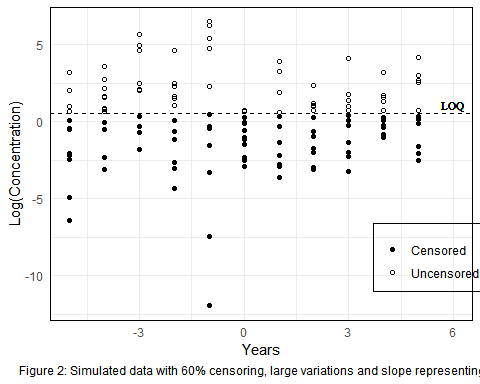
\includegraphics{Bachelor_Writing_files/figure-latex/unnamed-chunk-2-1.pdf}

\url{http://faculty.washington.edu/mlt/Thompson\%202003b.pdf} (Sec 4) -
Mimiced the environmental setting to be as close to the one for the
museum as possible. - Considered 1. 2. 3. (List) - \# of simulations
using MLE and substitution - Left censored - X and Y supposed to
represent \ldots{}.

We want a slope representing a 1\% yearly increase. Our model is
\(Y=e^{\beta_1 X + \epsilon}\) so when \(X\) goes to \(X+1\) we want
\(Y\) to go to \(Y\cdot 1.01\) hence
\(Y(x+1)=e^{\beta_1 (X + 1) + \epsilon} = e^{\beta_1 X + \epsilon}e^{\beta_1}=Y\cdot e^{\beta_1}\)
hence \(e^\beta_1=1.01\) so \(\beta_1=log(1.01)\) so in the log scale,
our slope is log(log(1.01)) : Probobly wrong

To choose variance for the individual fish error term, group\_by each
location, calculate standard deviations and pick lowest and highest.

To choose variances for year, do the same as for individual but also
group\_by YEAR, only pick locations that did analysis on individual
specimens, removing those that did analysis on a group of fish since
they only have 1-2 observations per year giving a bad estimate of yearly
variance.

The variances are calculated using the R functions from chapter 6 in the
environmental book.

What do I want to look at?! - Check for outliers? - Max difference - \%
in CI

Tips på analyser:
\url{https://onlinelibrary.wiley.com/doi/10.1002/sim.8086\#sim8086-fig-0005}

\subsection{Result}\label{result}

\subsection{Conclusion}\label{conclusion}

\begin{itemize}
\tightlist
\item
  EM-algorithm can stop at local maxima or sadle points, at sadle point
  the LH-fkn grows without bound.
\item
  Can, and should, try with higher (or no) limit of iterations if not so
  time heavy.
\item
  Test explicit starting values (based on what?)
\end{itemize}

\subsection{References}\label{references}

\begin{enumerate}
\def\labelenumi{\arabic{enumi})}
\item
  Helsel, D.R., 2006, Fabricating data: how substituting values for
  censored observations can ruin results, and what can be done about it.
  Chemosphere 65, pp.~2434--2439, doi:
  \url{https://doi.org/10.1016/j.chemosphere.2006.04.051}
\item
  Chung, C.F., 1990, Regression analysis of geochemical data with
  observations below detection limits, in G. Gaal and D.F. Merriam,eds.,
  Computer Applications in Resource Estimation. Pergammon Press, New
  York, pp.~421--433, doi:
  \url{https://doi.org/10.1016/B978-0-08-037245-7.50032-9}
\item
  Lee, T.L and Go, O.T, 1997, Survival Analysis in Public Health
  Research, vol.18, pp.~105-134, doi:
  \url{https://doi.org/10.1146/annurev.publhealth.18.1.105}
\item
  Chay, K.Y. and Honore, B.E. , 1998, Estimation of censored
  semiparametric regression models: an application to changes in
  Black--White earnings inequality during the 1960s. Journal of Human
  Resources Vol.33, pp.~4--38, doi: 10.2307/146313
\item
  Pinheiro, J.C and Bates, D.M, (2000), Mixed-Effects Models in S and
  S-PLUS (1. ed.), New York: Springer
\item
  Laird, N. M. and Ware, J. H. (1982). Random-effects models for
  longitudinal data. \emph{Biometrics}, Vol 38. (No. 4), pp.~963--974.,
  DOI: 10.2307/2529876
\item
  Bignert, A., Danielsson, S., Faxneld, S., Ek, C., Nyberg, E. (2017).
  Comments Concerning the National Swedish Contaminant Monitoring
  Programme in Marine Biota, 2017, 4:2017, Swedish Museum of Natural
  History, Stockholm, Sweden, Retrieved from the website of the Museum
  of Natural Historys:
  \url{http://nrm.diva-portal.org/smash/get/diva2:1090746/FULLTEXT01.pdf}
\item
  Eaton, M. L. (1983). Multivariate Statistics: a Vector Space Approach.
  John Wiley and Sons. pp.~116--117. ISBN 978-0-471-02776-8
\item
  Held, L, Bové, D.S, (2014), Applied Statistical Inference (1. ed.),
  New York: Springer
\item
  Dempster A. P., Laird N. M., Rubin, D. B. (1977), Maximum Likelihood
  from Incomplete Data via the EM Algorithm. \emph{Journal of the Royal
  Statistical Society. Series B (Methodological)}, Vol. 39, (No. 1) ,
  pp.~1-38, Retrieved from the website jstor:
  \url{https://www.jstor.org/stable/2984875?seq=1}
\item
  Thompson, M .L. and Nelson, K. P., (2003), Linear regression with Type
  I interval- and leftcensored response data. \emph{Environmental and
  Ecological Statistics} Vol. 10, 221--230. Retrieved from the website
  of the University of Washington:
  \url{http://faculty.washington.edu/mlt/Thompson\%202003b.pdf}
\item
  El-Shaarawi, A. H., Esterby, S.R.(1992), Replacement of censored
  observations by a constant: An evaluation. \emph{Water Research}, Vol
  26. (No. 6), pp.~835-844, doi:
  \url{https://doi.org/10.1016/0043-1354(92)90015-V}
\item
  Helsel, D.R., (2005), STATISTICS FOR CENSORED ENVIRONMENTAL DATA USING
  MINITAB AND R (2. ed.), Hoboken, New Jersey: John Wiley \& Sons,
  pp.~62-69, Inc., ISBN 978-0-470-47988-9(cloth)
\end{enumerate}

Vaida, F., Liu, L. (2009), Fast Implementation for Normal Mixed Effects
Models With Censored Response. \emph{Journal of Computational and
Graphical Statistics} Vol 18. (No. 4), 2009 - Issue 4 , doi:
\url{https://doi.org/10.1198/jcgs.2009.07130}

\end{document}
